%% ----------------------------------------------------------------------------
% CVG SA/MA thesis template
%
% Created 03/08/2024 by Tobias Fischer
%% ----------------------------------------------------------------------------
\chapter{Appendix}

% -------- Instructions for writing the appendix section:
% In the appendix, list the following material: 

% \begin{itemize}
 % \item Data (evaluation tables, graphs etc.)
 % \item Program code
 % \item Further material 
% \end{itemize}

\section{Instance Segmentation}
\label{sec:appendix_segmentation}

\paragraph{Metrics.}
Segmentation quality is important to accurately separate dynamic humans from the static background. We therefore measure segmentation quality using intersection-over-union (IoU), recall, and F1 score.

\subsection{Results}
\begin{figure}[!ht]
    \centering
    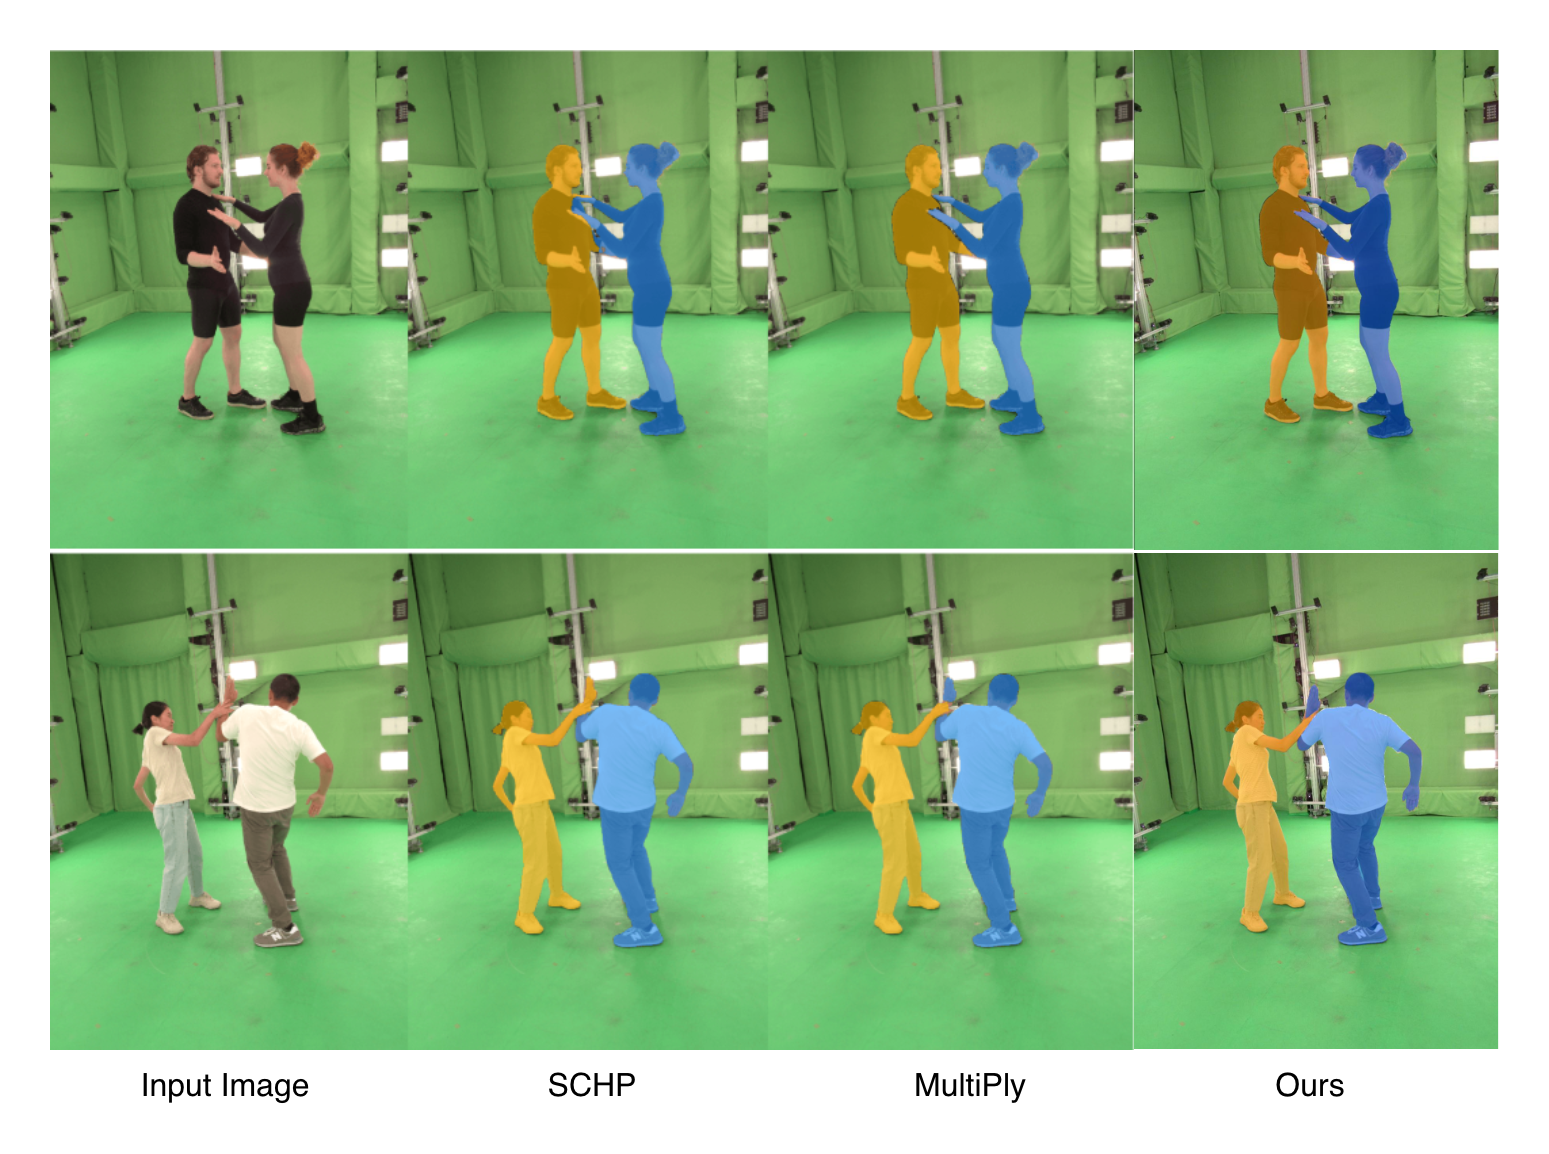
\includegraphics[width=1.0\textwidth]{figures/qual_segment_comp.drawio.png}
    \caption{\textbf{Qualitative instance segmentation comparison}. We adapt the figure from MultiPly \cite{multiply} and added our segmentation results for comparison on chosen scenes from Hi4D. For each method, we show RGB frame overlaid with predicted instance masks.}
    \label{fig:qual_instance_segm_comp}  
\end{figure}

\begin{table}[!ht]
  \centering
  \small
  \setlength{\tabcolsep}{7pt}
  \begin{tabular}{l
      S[table-format=1.3]
      S[table-format=1.3]
      S[table-format=1.3]}
    \toprule
    \textbf{Method} & \multicolumn{1}{c}{\textbf{IoU} $\uparrow$} & \multicolumn{1}{c}{\textbf{Recall} $\uparrow$} & \multicolumn{1}{c}{\textbf{F1} $\uparrow$} \\
    \midrule
    MultiPly (Init.) & 0.943 & 0.975 & 0.984 \\
    MultiPly (Progressive) & 0.963 & \textbf{0.985} & \textbf{0.990} \\
    Ours (using SAM3) & \textbf{0.974} & 0.982 & 0.987 \\
    \bottomrule
  \end{tabular}
  \caption{\textbf{Human instance segmentation results on Hi4D.} Best results are in bold.}
  \label{tab:segmentation_results_hi4d}
\end{table}

We compare our mask segmentation quality to MultiPly, which reports results for both its initial masks from SAM1 \cite{sam1} and its progressively refined masks during training. In contrast, we do not refine masks during training and rely on the initial masks from SAM3 \cite{carion2025sam3segmentconcepts}. All methods achieve strong scores, with our method obtaining the best IoU, while MultiPly's progressive masking achieves slightly higher recall and F1. This suggests different error modes: SAM3 tends to produce cleaner average overlap, while progressive refinement reduces missed foreground pixels. Overall, segmentation quality is strong and is unlikely to be the main bottleneck, although small boundary errors can still affect downstream rendering and reconstruction.

Figure \ref{fig:qual_instance_segm_comp} shows representative failure cases of our SAM3-based instance segmentation compared to MultiPly. In the top row, our method assigns part of the orange person's left arm to the blue person; in the bottom row, part of the orange person's right hand is similarly assigned to the blue person. These errors are primarily instance-level mix-ups at contact or occlusion boundaries. In practice, they are less critical for our main objective of separating dynamic humans from the static background, which both methods achieve reliably.
